\documentclass{article}

\usepackage{amsfonts,graphicx, picins}

\setlength{\textwidth}{17cm} \setlength{\textheight}{9in}
\oddsidemargin=-0.2cm \topmargin=-1.3cm
\renewcommand{\thesection}{\Alph{section}}
\renewcommand{\thepage}{\thesection-\arabic{page}}

\title{Qualitative Comparison of Coding Languages\\ used for Image Synthesis}

\author{Christopher Potter}

\begin{document}

\maketitle

\begin{abstract}
 In this thesis four different computer programming languages, C++, Python, Processing and Pixar's Renderman, will be used to realize four different rendering programs.  The goal is to analyze the main challenges in implementing with each language and qualitatively evaluate each implementation once completed.  A set of ``ray tracing milestones" will be established so that each language can address the challenges unique to that language.
\end{abstract}
%%%%%%%%%%%%%%%%%%%%%%%%%%%%%%%%%%%%%%%%
%%%%%%%%%%%%%%%%%%%%%%%%%%%%%%%%%%%%%%%%
\begin{figure}[htbp]
\begin{center}
\begin{tabular}{cccccc}
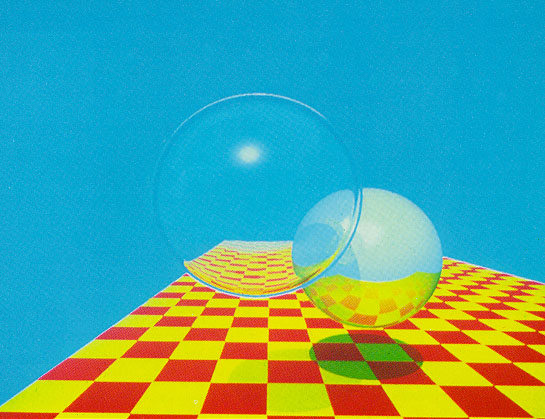
\includegraphics[height=2.00in]{images/turner}&
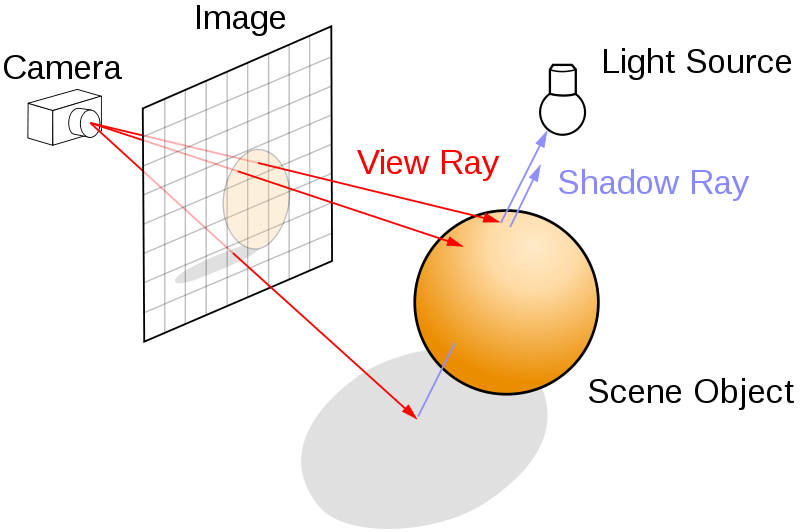
\includegraphics[height=2.00in]{images/Ray_trace_diagram}\\
(a) Turner, 1980 & (b) Ray Tracing Diagram \\
\end{tabular}
\caption{Examples of early ray tracing: (a) Image from first ray tracing paper by Turner Whitted. (b) and a simple breakdown of the ray tracing process.}
\label{fig:regions}
\end{center}
\end{figure}

\section{Motivation and Introduction}
3D Rendering, the processing of creating 2D images from 3D geometric shapes with the use of photorealistic/non-photorealistic effects on a computer, is one of the fundamental building blocks for 3D graphics image production.  When rendering images for photorealism, understanding how different effects are mathematically represented by the computer provide an informed freedom to effectively manipulate the given render controls to produce a desired result faster.  Industry professionals encourage lighting artists to gain experience writing rendering programs for this reason.

Writing a rendering program can be very intimidating for an artist. Rendering programs consist of two fundamental parts, theory and implementation.  The complex vector/matrix math theory to compute intersections within the 3D scene can be difficult to understand by itself.  Coupling those theories with proper computer language jargon can multiply the difficulty.  In addition to remembering the linear algebra, artists need to worry about code syntax and segmentation faults(generally an attempt to access memory that the CPU cannot physically address), which can be demoralizing to even the most experienced computer scientist.  Rather than gaining experience/experimentation in the mathematics of image synthesis, artists can become distracted from the task at hand by focusing on the logistics of implementing unnecessary code.  This thesis will attempt to provide guidelines to introduce programming languages and techniques related to rendering to artists so they can spend less time on the implementation aspects of the process and more time on the theoretical experience of image synthesis.



\section{Background/Literature Review}
There are a variety of approaches to producing a rendering program.  The fundamentals of most rendering programs lie in ray casting and ray tracing.  For this thesis ray tracing and ray casting will both be described as the process of generating an image by tracing the path of virtual rays from an eye source through pixels in an image plane and simulating the effects of its encounters with virtual objects/lights. Each will be differentiated further by their illumination models, or the shading algorithms used to interact with light rays. \piccaption[]{Ray Casting}\parpic[1]{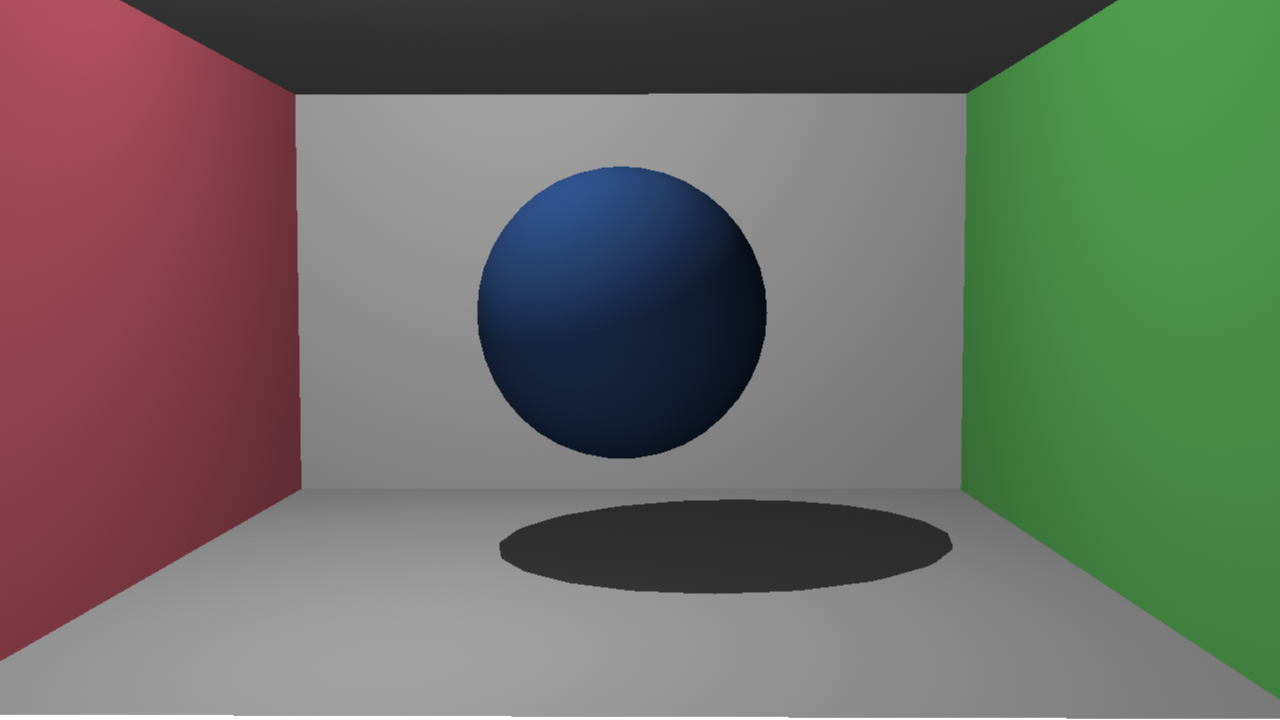
\includegraphics[width=2.0in]{images/rayCasting}}

Ray casting, a term first introduced by Scott Roth in 1982, is the process of casting rays into a 3D scene, finding the closest intersection from the eye/camera through boolean operations and returning the color value of that object\cite{Roth1982}. By emulating different properties of light based off of the cosine of the normal vector and the normalized vector from the hit point of the object to a light, semi-realistic results were produced\cite{Phong1975,gouraud1971,Blinn:1977,Cook:1987}.  Other more cartoon-ish effects were produced using similar methods as well, most notably Gooch and Gooch shading\cite{Gooch1998}. For this thesis, ray casting will be categorized under direct illumination, a term meaning only illumination from a light in the 3D environment will be calculated on the objects final color and shading(Figure 2).  This also includes shadowing information, which is just light obstructing the ray path from a light to the hit point.

\piccaption[]{Ray Tracing}\parpic[r]{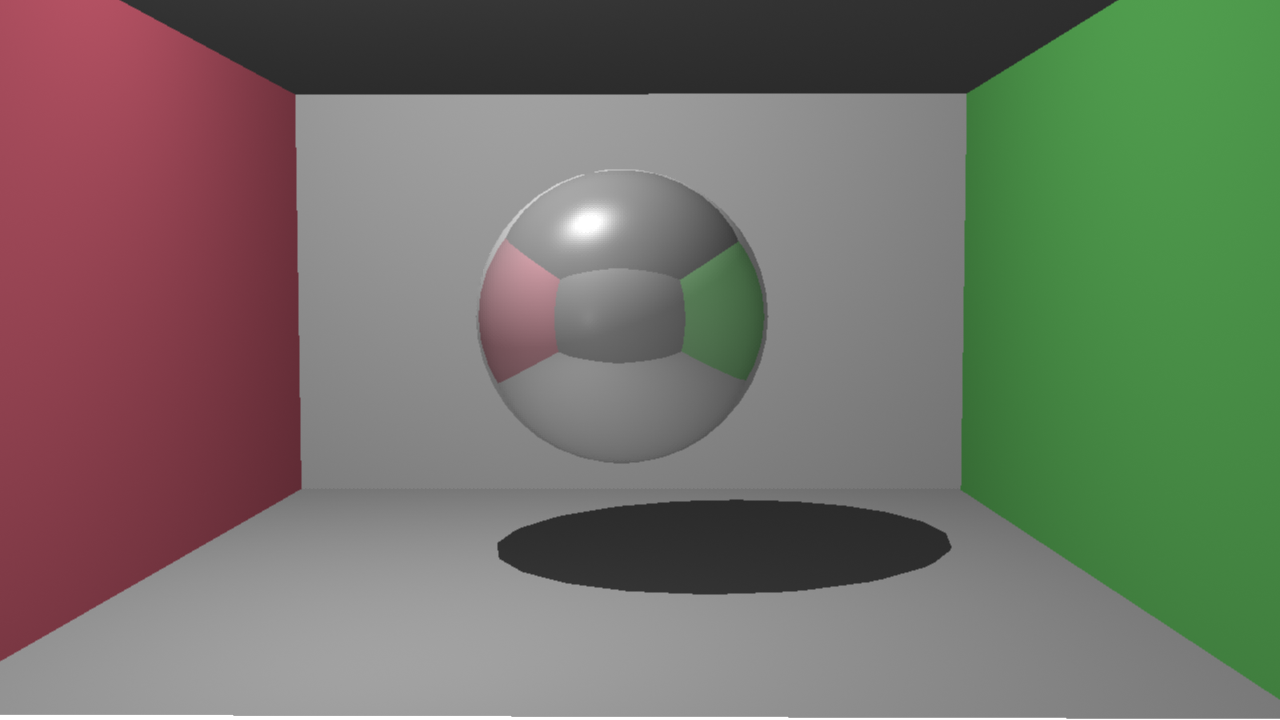
\includegraphics[width=2.0in]{images/rayTracing}}To make more realistic reflections and refractions in rendered images, a recursive process needs to be implemented\cite{Whitted1980}.  This process, which we will refer to as ray tracing, allows surfaces to recursively call shading algorithms from objects virtually to infinity, producing hyper realistic interactions of light off of objects(Figure 3).  This approach can be categorized under indirect illumination, or the shading model will be defined not only by the lights in the scene from direct illumination but also from shading information from other objects in the scene.  Reflection calculates an objects color from other diffuse objects in the scene.  At the point of intersection with an object, another ray is calculated and the ray-intersection process starts over again, until a color is returned for the surface.  Refraction is the same, except the ray is transmitted through the object.

Once ray tracing of reflections has occurred, one can start a process called ``distributed ray tracing", coined by Robert Cook, Thomas Porter and Loren Carpenter\cite{cook1984}. Simply put from Cooks paper when referring to the rays traced in a ray tracer:

\begin{quote}
Ray direction, however, have been determined precisely, and this has limited the capabilities of ray tracing.  By distributing the direction of the rays according to the analytic function they sample, ray tracing can incorporate fuzzy phenomena.
\end{quote}

To produce a fuzzy reflection, or glossy reflection, Cook suggests to ``jitter" the reflection vector every sample.  Doing the same on a refraction vector will produce a translucent effect.  When jittering the starting position of a ``camera" ray in the rendering program, you will get a depth of field effect, which is the distance between the nearest and the furthest objects that give an image judged to be in focus in a camera.  And finally, in an animation path, when jittering the placement of an object between key positions of the object, you will get motion blur effects. All these things are considered distributed ray tracing.

 Indirect illumination also includes diffuse reflections.  This includes all radiosity effects as well.  Every material in nature, even diffuse objects, have some sort of reflection or influence from other objects in its environment.  Goral et. al. from Cornell University identified a way to model the indirect lighting effects from color bleeding or environmental illumination of neighboring objects, which emulates this diffuse reflection\cite{Goral:1984}.  Using Goral's algorithm can give us a variety of indirect illumination effects.

Ambient occlusion, an approximation of the way light radiates in real life, especially from non-reflective surfaces, can be accomplished by transmitting a set number of ``diffuse rays" from each hit point and determining a ratio of intersected rays to total rays cast off the surface.  This will create a black and white image darkest at the parts of the image where objects are closest together.  Color bleeding or global illumination accomplishes this same task, but rather than summing the total ray cast, it averages the diffuse shading information for each ray cast from the hit point.  Averaging the specular shading information from each sample cast from the hit point gives us either a reflective or refractive caustic.  All these effects are shown in Figure 4.

\begin{figure}[htbp]
\begin{center}
\begin{tabular}{cccccc}
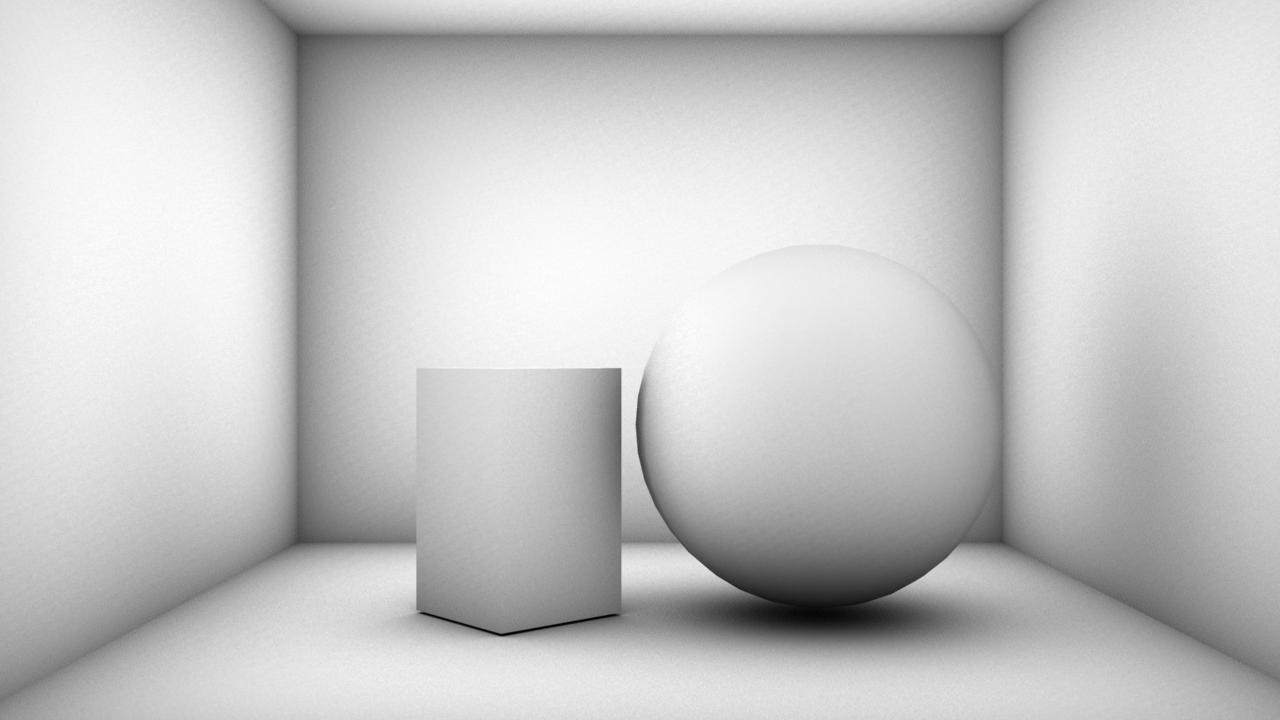
\includegraphics[height=1.15in]{images/aOcclusion}&
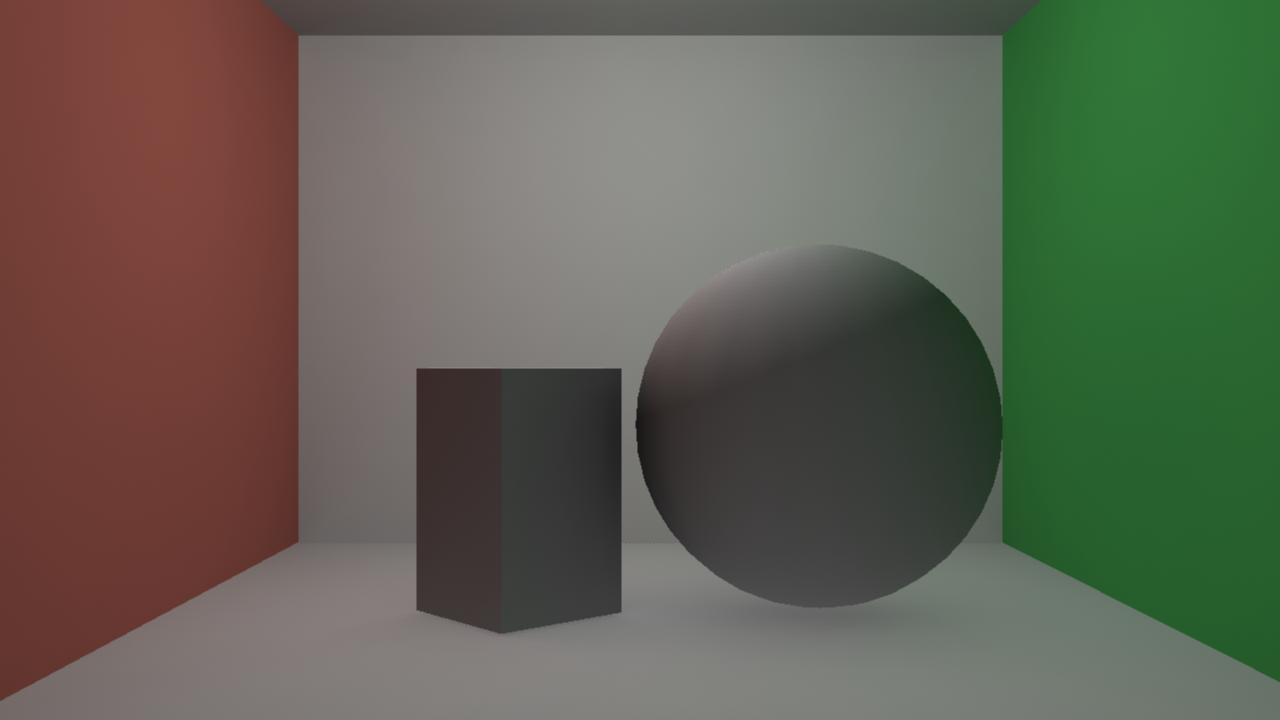
\includegraphics[height=1.15in]{images/globalIll}&
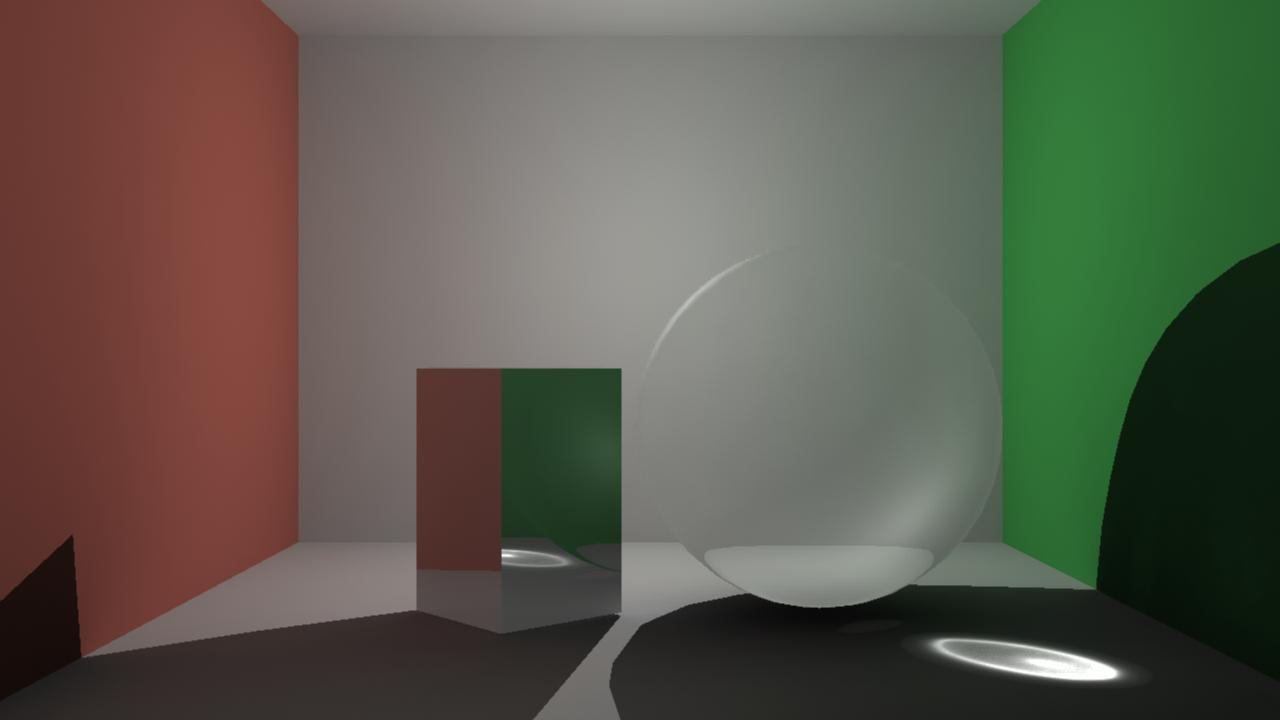
\includegraphics[height=1.15in]{images/caustics}\\
(a) Ambient Occlusion & (b) Global Illumination & (c) Caustics \\
\end{tabular}
\caption{Examples of diffuse reflections categorized under indirect illumination.}
\label{fig:regions}
\end{center}
\end{figure}

Direct illumination, distributed ray tracing and indirect illumination make up the bulk of image synthesis programs and will be three out of four milestones for this thesis.
\section{Problem}
Many students automatically use C++ code when trying to implement a image synthesis program.  C++ can be a very intimidating programming language that might be too complex and syntax heavy, causing students to get caught up in the coding process rather than the desired outcome which is learning the mechanics of a ray tracer.  In this we hypothesize that Python, Processing or Renderman will provide a better platform due to the shallower learning curve and intuitive nature of these languages.
\section{Method}
The process of image synthesis can be broken up into distinct sections: preliminary preparations, direct illumination, distributed ray tracing, and indirect illumination.

Preliminary preparations refers to necessary classes or data structures needed to perform basic math operations or image reading/writing functions crucial to creating/saving ray traced images.  This can also refer to any outside knowledge of a language needed, for instance makefiles(the declarative text file that informs computer systems how to ``build" an executable program) and compilers needed to run C++ code.  Direct illumination refers to ray casting for this thesis.  Ray casting is the simplified form of ray tracing that accounts for light intersections but does not include reflections or refractions.  Distributed ray tracing can be described as including the reflection and refraction capabilities of material properties, along with altering techniques of glossiness and translucency.  Distributed ray tracing also involved camera depth of field and motion blur for animation, since fundamentally they involve the same "jittering" process as glossiness and translucency.  Indirect illumination is anything beyond the ray tracing point.  These include ambient occlusion, color bleeding, environmental illumination and caustic effects.

There are many different computer languages to choose from.  Rendering can be very computationally heavy.  For this reason, until recently when computer technology has become more advanced, ray tracing practices are only used in places where real-time graphics production is unnecessary, such as animation and effects studios.  While speed is important in the animation industry, and a fun challenge for aspiring computer scientists, in regards to the process of learning for an artist, C++ may be too complex for non-computer scientists interested in learning the ray tracing process.

Python developers boast of its clear, readable syntax, intuitive object orientation and high level dynamic data types. The Rochester Institute of Technology, a school with a popular undergraduate computer science major, has started teaching Python rather than Java to introductory students interested in computer science.  The Python website also lists 34 confirmed Universities in the United States that teach python to students, some teaching specifically to non-computer science majors. This suggests that Python is easier to grasp and quicker to start developing content within.  We suggest this is because of the shallow learning curve to the syntax and the ability for high level concepts to be introduced earlier because of built in modules.

Processing, based off of Java, tries to bridge the gap between scripting and artistic creation by wrapping a lot of functionality in a Graphical User Interface(GUI) and an extensive functionality library\cite{glassner2010processing}.  Initially Processing was developed as a software sketchbook and to teach fundamentals of computer programming within a visual context.  This language is specifically taught to students/artists at a number of universities, including New York University, UCLA, Miami University's Armstrong Institute for Interactive Studies, and the University of Washington's Applied Physics lab, which suggests it is intuitive to use and quick to produce results.  Many projects accomplished with Processing are mathematically based, so bridging the gap into ray tracing is not farfetched.

Pixar has established it's own rendering language, which involves a dual process, a RenderMan Interface Bytestream (RIB file), which sends scene data to the RenderMan rendering engine, and RenderMan Shading Language (RSL), which is a procedural shading language that enables creation of custom shaders based off of the built-in shading functions established within the RenderMan engine \cite{cook1984shade}.  This process is a camera projection process, which is not ray tracing, but might still prove useful to understand some aspects of the rendering process and the shading process.  In this thesis we hypothesize that it will be too simple to accomplish the ray-tracing theory tasks since RenderMan encapsulates a lot of shading capability within pre-existing functions, so the learning process for RSL and RIB generation will not be beneficial to understand the fundamental ray casting theory, but might provide insight to how shading works.
\section{Initial Findings}
So far, the research has found that the Processing language, while similar to Java, has been extremely easy to use and produce the desired effects of the fundamental ray tracing projects. However, the compilation time of each test image is significantly longer than it would take a C++ program to complete.  The initial Processing projects take minutes compared to C++, which takes seconds. One reason for this may be Processing wraps the Java implementation, something is occuring ``under the hood" that might be making the projects compile slower than it normally would.  The Python language also takes a very long time to generate images, which is expected since it is an interpreted language.  The simplest project for Python compiles in roughly ten minutes.  A new approach will be needed to assess the viability of Python as an image synthesis language without over complicating the scripting process.  As part of the thesis, a survey of compilation time per project per language will help to determine if the compilation time trends equivalently.

An exploration of the RenderMan engine thus far has proven frustrating.  Additional research into documentation or instructional resources needs to be done to determine the viability of using the language.  Renderman has created a language that encompasses the mathmatical process of ray casting, so the fundamentals of rendering implementation are unable to be taught through this language.  So far, this language does provide a brief overview of how a shader should work and helps to break down the fundamentals of shading and scene descriptions.  So while the learning curve might be difficult, knowing how RenderMan establishes scenes and processes a shader is beneficial to applying to a self made image synthesis program.
\section{Conclusion}	
Four ray tracers will be written in C++, Python, Processing and Renderman.  The goal of the research is to identify the most appropriate candidate language for implementing raytracing theory for artists.  Along with nicely rendered images from each of the different languages, a qualitative analysis of each language and the effort made to accomplish each milestone will be recorded as completely as possible.

It is the goal of this research to make scripting the concepts of raytracing more accessible to artists.  This research should provide the building blocks towards teachable resources for students to reference and build a deeper understand of raytracing theory.  A generic code-base with actual coding resources for students to reference outside of the physical thesis document itself will be established.
\bibliographystyle{plain}
\bibliography{bibliography}

\end{document}


